\documentclass[twocolumn, a4paper]{article}
\fontsize{10.5}{10}\selectfont
\def\figsize{0.50\textwidth} 

% ------------------------------------------------------------------
% Importação do arquivo de definições
\usepackage{graphicx} % pacote para adição de figuras no texto
\usepackage{multirow} % textos e tabelas com múltiplas linhas
\usepackage{multicol} % textos e tabelas com múltiplas colunas
\usepackage{cuted} % definir espaçamento do titulo
\usepackage{fancyhdr} % pacote usado para o rodapé
\usepackage{mathptmx} % Fonte da família Times
\usepackage{titling} % ajuste de título e subtítulos
\usepackage{titlesec} % ajuste de título e subtítulos mesmo diretório
\usepackage[T1]{fontenc}

\usepackage[utf8]{inputenc}
%----------------------------------------------------------------------
% formatação em itálico da legenda da figura
\usepackage{caption}
\captionsetup[figure]{format=plain, textfont=it}{}
% --------------------------------------------------------------------
% Define o espaçamento superior antes do início do título
\setlength{\droptitle}{-6em} 
%----------------------------------------------------------------------
%----------------------------------------------------------------------
% Definição do texto e numeração das seções e legenda de figuras e tabela
\titlelabel{\thetitle.\vspace{2pt}}
\titleformat{\section}
  {\normalfont\large\bfseries\filcenter}{\thesection.}{0.5em}{}
\titleformat{\subsection}
  {\normalfont\normalsize\itshape}{\thesubsection.}{0.5em}{}
\titlespacing{\section}{0pt}{10pt}{5pt}

\renewcommand{\thesubsection}{\Alph{subsection}}
\renewcommand{\thesection}{\Roman{section}}
\renewcommand{\figurename}{Fig.}
\renewcommand{\tablename}{TABELA}
\graphicspath{{Figuras/}}
%----------------------------------------------------------------------
% Retira a numeração automática de rodapé
\pagenumbering{gobble}
%----------------------------------------------------------------------
% Rodapé da primeira página
\fancypagestyle{specialfooter}{%
  
  \fancyhf{}
  \renewcommand\headrulewidth{0pt}
  \fancyfoot[C]{Seminários de Microeletrônica do Paraná \\
Curitiba, Brasil}
}
%----------------------------------------------------------------------
%----------------------------------------------------------------------
% Definição da margem das páginas
\usepackage{geometry}
 \geometry{
     a4paper,
     left=16mm,
     top=19mm,
     right=16mm,
     bottom=25.4mm
 }
%----------------------------------------------------------------------
% ---------------------------------------------------------------------
% Titulo do texto
\title{
    \begin{minipage}[c]{0.3\textwidth} 
          
\includegraphics[width=\textwidth]{Semicro_title.png} 
    \end{minipage}\begin{minipage}[c]{0.7\textwidth} 
             \begin{center}
                \Huge
                 Pré-distorcedor digital descrito em linguagem VHDL e baseado em polinômio com memória.\\
                \vspace{20pt}
                \Large
                  Leonardo de Andrade Santos, Sibilla Batista da Luz Franca, Eduardo Gonçalves de Lima \\
                  \normalsize
                  \textsuperscript{1} Universidade Federal do Paraná, Curitiba, Brasil \\
                  leonard.andrade@ufpr.br
             \end{center}
    \end{minipage}
}

% Define o tamanho do espaço vertical abaixo do título
\date{\vspace{-8em}}
% Define a separação entre as colunas
\setlength\columnsep{2em}


% ------------------------------------------------------------------
% Início do documento
\begin{document}

% ------------------------------------------------------------------
\begin{strip}
	\vspace*{\dimexpr-\baselineskip-\stripsep\relax}
	%\centering
	\maketitle
	\vskip\baselineskip
	\noindent %\makebox[\textwidth]{\rule{1.1\paperwidth}{0.4pt}} Linha horizontal
	\vskip\baselineskip
\end{strip}
% EDITAR A FIGURA 1  AUMENTAR A FIGURA APROXIMANDO OS BLOCOS
%CORRIGR NUMERO DE PAGINAS
%TIRAR FONTE : AUTOR
%REORDENAR LISTAS DE REFERÊNCIAS CONFORME APARECE NO TEXTO
% ------------------------------------------------------------------
% Nota de rodarezzé da primeira página
\thispagestyle{specialfooter}
% ------------------------------------------------------------------
% Resumo (definição em itálico e negrito)
\vspace{3pt}\textbf{\textit{Resumo - A evolução da comunicação sem fio impulsionou aplicações como IoT, onde a eficiência energética é crucial para dispositivos móveis e estações de rádio. No entanto, essa eficiência compromete a linearidade dos amplificadores de potência (PA), afetando modulações de fase e amplitude. Sendo assim, uma alternativa para contornar esse obstáculo é a implementação de um (DPD) em cascata com um PA. Portanto, este trabalho propõe a implementação de um código em VHDL para processar as características de transferências inversa de um amplificador de potência em tempo real, minimizando não linearidades e consumo de energia. A modelagem foi feita inicialmente em software e implementada em FPGA (Field-Programmable Gate Array) para validação e análise de desempenho. Durante o desenvolvimento, testes e análises foram realizados com um polinômio de memória de segundo grau e um sinal de amostra memorizado, mostrando uma redução efetiva nas distorções do PA. Foi utilizada a métrica de Erro Quadrático Médio Normalizado (NMSE - Normalized Mean Squared Error) para quantificar a qualidade da modelagem implementada. O NMSE de -23,57 dB mostrou eficiência na redução de distorções. Assim a etapa seguinte consistiu na modelagem do PA em vírgula fixa, a fim de atingir o NMSE mais próximo do atingido em vírgula flutuante com a menor resolução em bits, visando alcançar o melhor desempenho em hardware. A modelagem em vírgula fixa com 8 bits aprimorou o desempenho. Por fim, o modelo foi implementado em hardware na FPGA Virtex5 XC5VLX50T, utilizando um total de 150 registradores, 692 LUTs e 4 unidades DSP48E, operando a uma frequência de 61,5 MHz.}}
% ------------------------------------------------------------------

\section{INTRODUÇÃO}
A evolução dos sistemas de comunicação móveis, impulsionada pela crescente demanda por comunicações mais rápidas e eficientes, tem levado à implementação de uma variedade de serviços, incluindo aplicações multimídia, desenvolvimento web e aplicações IoT \cite{John2016}. No entanto, essa evolução também trouxe desafios significativos, como a necessidade de melhorar a eficiência energética, tanto para dispositivos móveis, visando aumentar a autonomia da bateria, quanto para estações de rádio base, visando reduzir o consumo de energia devido às perdas de calor. Para atender a essas demandas, estratégias de modulação que alteram tanto a fase quanto a amplitude de ondas portadoras em radiofrequência se tornaram essenciais \cite{Kenington2000}. Além disso, a modulação na amplitude requer linearidade na transmissão para evitar erros e interferências na comunicação entre usuários vizinhos \cite{Cripps2006}. Essa complexa tarefa recai sobre o projetista do PARF (Amplificador de Potência de Rádio Frequência), que enfrenta o desafio de desenvolver um hardware eficiente em termos energéticos e linear ao mesmo tempo, uma vez que esses dois objetivos podem entrar em conflito \cite{Chavez2018}. Uma solução para contornar esse desafio é a implementação de um pré-distorcedor de Sinais Digital em Banda Base, que visa compensar a distorção causada pelo PARF \cite{Cripps2006}. O DPD (Pre-distorcedor Digital) é conectado em cascata ao PARF e requer um modelo de alta precisão e baixa complexidade computacional para representar as características de transferência direta e inversa do PARF. Existem duas abordagens para modelar o PARF: modelos físicos, que são detalhados e computacionalmente complexos, e modelos empíricos, que se baseiam em medições de entrada e saída do PARF, com menor complexidade computacional, mas com uma possível diminuição da precisão. Devido às exigências rigorosas de frequência de operação, a paralelização das operações torna-se essencial, e as FPGAs (Matriz de Portas Programáveis em Campo) emergem como uma alternativa viável para a implementação de circuitos pré-distorcedores \cite{Pedroni2010}. As FPGAs são dispositivos lógicos programáveis que permitem a reconfiguração física de componentes de eletrônica digital, acelerando processos e suportando operações paralelas e sequenciais. 
Neste contexto, este projeto foi planejado com o objetivo geral de construir e validar um código em linguagem de descrição de hardware capaz de processar, em tempo real, as características de transferência inversa de um amplificador, reproduzindo suas não linearidades. Além disso, o código deve ocupar a quantidade mínima de recursos lógicos do circuito digital que irá sintetizá-lo, visando à redução do consumo de energia. Para atingir esse objetivo, o trabalho foi desenvolvido com base nos seguintes objetivos específicos: modelar com precisão o amplificador de potência (PA) em software; modelar o pré-distorcedor digital (DPD) em software a partir da modelagem do PA e implementar o DPD em hardware utilizando uma linguagem de descrição de hardware (HDL).



\section{MODELAGEM MATEMÁTICA}
\subsection{Séries de Volterra}

Segundo \cite{Gonçalves2009} série de Volterra pode ser vista como uma extensão multidimensional da série de Taylor para sistemas dinâmicos. A modelagem começa com a representação do sistema através de uma série infinita de integrais convolucionais, onde cada termo da série corresponde a uma ordem de não linearidade e memória.

A saída \( y(t) \) de um sistema pode ser expressa pela equação \ref{eq:Volterra}: \begin{equation}
	y(t) = h_0 + \sum_{n=1}^{\infty} \int_{-\infty}^{\infty} \cdots \int_{-\infty}^{\infty} h_n(\tau_1, \tau_2, \ldots, \tau_n) \prod_{i=1}^{n} x(t - \tau_i) \, d\tau_i
	\label{eq:Volterra}
\end{equation} onde \( h_n \) são os núcleos de Volterra, que caracterizam a resposta do sistema para a \( n \)-ésima ordem de não linearidade e \( x(t) \) é a entrada do sistema.

Os núcleos de Volterra \( h_n \) são funções de várias variáveis que capturam a dinâmica do sistema em diferentes ordens. Para a maioria das aplicações práticas, a série é truncada para incluir apenas um número finito de termos, já que a identificação de todos os núcleos de uma série infinita é impraticável.

\subsection{Polinômio de memória}

Um modelo simples, utilizado na modelagem comportamental simplificada das séries de Volterra considerando apenas componentes unidimensionais\footnote{Cada termo do somatório é composto por amostras no mesmo instante, por exemplo: $x(n)|x(n)|,x(n - 1)|x(n - 1)|$; termos bidimensionais são compostos por amostras em instantes de tempos distintos, como por exemplo: $x(n)|x(n - 1)|$} é o MP, que é um modelo compacto, de baixo custo computacional e linear em seus parâmetros. O MP gera baixo erro quando aplicado à PAs que apresentam pouco efeito de memória. O DPD e pós distorsor apresentam característica inversa a do PA \cite{Schuartz2017}, portanto o mesmo modelo pode ser utilizado. A equação \ref{eq:mp} apresenta o MP conforme é ilustrado por \cite{Schuartz2017}: 

\begin{equation}
	y(n) = \sum_{p=1}^{P} \sum_{m=0}^{M} h_{p,m} x(n - m) \left| x(n - m) \right|^{p-1}
	\label{eq:mp}
\end{equation}

Como a proposta do trabalho é a implementação em hardware desse modelo, torna-se necessário paralelizar operações aritméticas de forma a alcançar uma taxa de operação que satisfaça a norma regulamentadora. Nesse contexto, as FPGAs apresentam-se como uma alternativa viável para a implementação de circuitos pré-distorcedores.

\section{IMPLEMENTAÇÃO EM SOFTWARE} \label{sec:implsoft}
Nesta etapa, foi implementado o modelo DPD em software utilizando Python, com sinais de entrada e saída de um amplificador de potência classe AB baseado em HEMT GaN. O amplificador foi excitado por um sinal de 900 MHz modulado por WCDMA 3GPP, com largura de banda de aproximadamente 3,84 MHz. Os dados foram coletados usando um VSA Rohde \& Schwarz FSQ a 61,44 MHz de taxa de amostragem \cite{Bonfim2016}. 

A seguir, foi calculada a estimativa do sinal utilizando números de vírgula fixa e validada com o NMSE. Para isso, os dados foram divididos em conjuntos de extração e validação. A matriz de regressão foi calculada com os dados de extração para obter os coeficientes do polinômio de memória. O modelo foi validado com os dados de validação, resultando em um NMSE de -23,57 dB para um polinômio de 2° grau com uma amostra memorizada.

O algoritmo foi então ajustado para trabalhar com números em vírgula fixa, buscando a menor resolução possível e o menor NMSE simulado, o que exigiu a readequação dos resultados entre as multiplicações para manter a resolução inicial.

\section{IMPLEMENTAÇÃO EM FPGA}
Essa etapa consiste na implementação do DPD em FPGA, onde é necessário realizar paralelizações nas operações aritméticas, separando os processos de potência, multiplicação e soma em etapas distintas. A cada ciclo de clock, duas operações são realizadas em paralelo: o sinal atual é elevado ao quadrado e registrado, enquanto ocorre o somatório do produto entre os sinais do mesmo instante de tempo e seus respectivos coeficientes. Esse processo é repetido P vezes, de acordo com os \( P \) graus do polinômio de memória. Como resultado, a saída do DPD é incompleta durante os primeiros \( P \) ciclos de clock, pois, nesse período inicial, o cálculo é realizado com base em entradas de sinais anteriores que ainda não ocorreram, resultando em uma saída incompleta.

\section{RESULTADOS}
\subsection{Modelagem do PA}

Para fazer a modelagem em software foi utilizada a linguagem de programação Python. Para isso, separou-se os dados citados na seção \ref{sec:implsoft}, em dados de extração e dados de validação, os quais são utilizados para extração dos coeficientes do modelo do MP e validação do modelo encontrado, respectivamente. Para fazer a validação do modelo utilizou-se a métrica do NMSE, que consiste em calcular o erro quadrático médio do valor medido pelo VSA (Analisador de Sinal Vetorial) para o valor calculado pelo modelo. Portanto, quanto menor o NMSE mais fiel é o modelo do PA. Nesta etapa obteve-se um NMSE de -23.57 dB, para cálculos em vírgula flutuante, onde o resultado está presente no gráfico da figura \ref{fig:modelopafloat}.

\begin{figure}[htbp]
    \centering
    \captionsetup{justification=centering}
    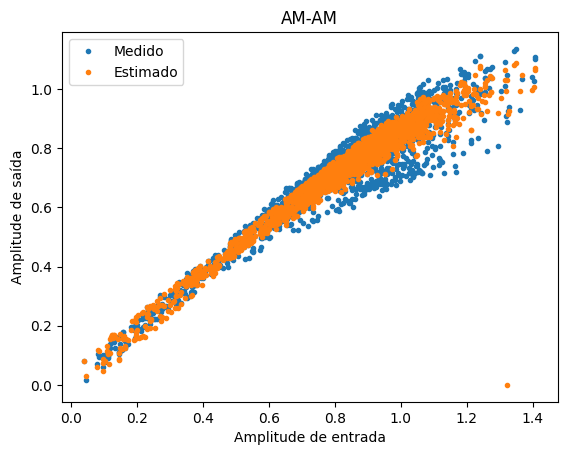
\includegraphics[width=\figsize]{modeloPAfloat.png}
    \caption{Modelo do PA em vírgula flutuante}
    \label{fig:modelopafloat}
\end{figure}

\subsection{Definição do número de bits}

Após concluída a modelagem matemática, realizou-se a modelagem do PA para então ser feito o levantamento da quantidade de bits necessários para a implementação do DPD em hardware minimizando os erros de quantização. 
Para isso foi necessário refazer a extração dos coeficientes, mas desta vez com os dados normalizados para valores de 0 a $2^{bits}$.  
O resultado desse levantamento está presente no gráfico na figura \ref{fig:bits}.

\begin{figure}[htbp]
    \centering
    \captionsetup{justification=centering}
    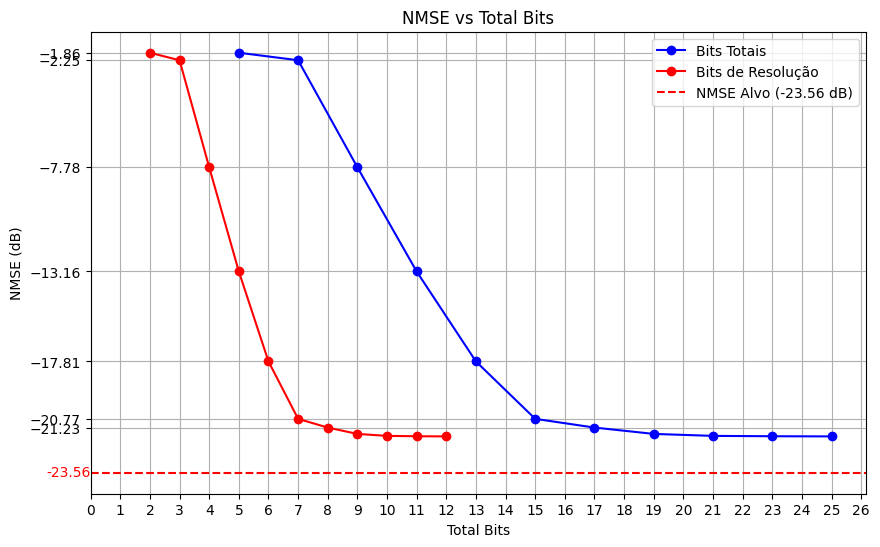
\includegraphics[width=\figsize]{bits.png}
    \caption{Gráfico Número de bits x NMSE}
    \label{fig:bits}
\end{figure}

Neste gráfico observa-se duas curvas, a curva em azul apresenta a quantidade total de bits contando com os bits de overflow necessárias para as operações de multiplicação, enquanto a curva em vermelho representa a quantidade de bits de resolução do sinal. Analisando este gráfico observou-se que não existem ganhos significativos no erro a partir de 8 bits, portanto foi feita a modelagem do PA utilizando uma resolução de 8 bits. O resultado alcançado está ilustrado pela figura \ref{fig:modelopa}.

\begin{figure}[htbp]
    \centering
    \captionsetup{justification=centering}
    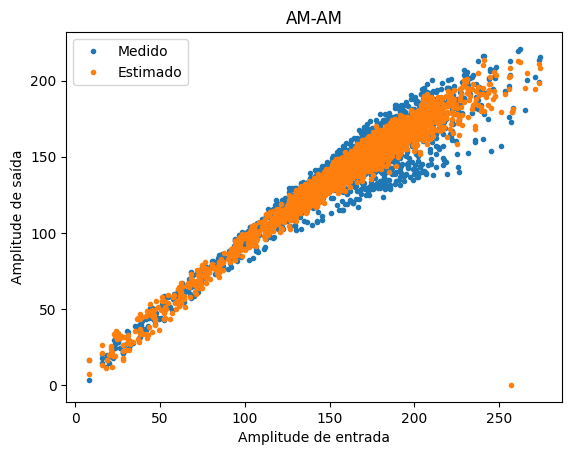
\includegraphics[width=\figsize]{modeloPA.png}
    \caption{Modelo do PA em vírgula fixa}
    \label{fig:modelopa}
\end{figure}

\subsection{Modelagem do DPD}
A partir dos resultados obtidos foi possível fazer a modelagem do DPD, para isso foi feito o mesmo processo de modelagem do PA, porém para alcançar a característica de transferência inversa do PA foi invertido a ordem dos dados de entrada e saída para extração dos coeficientes do DPD. O resultado desta modelagem está ilustrado pela figura \ref{fig:modelodpd} a seguir.

\begin{figure}[htbp]
    \centering
    \captionsetup{justification=centering}
    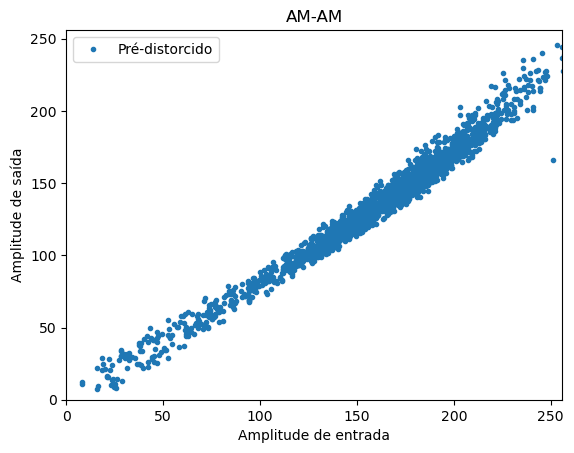
\includegraphics[width=\figsize]{modelodpd.png}
    \caption{Modelo do DPD em vírgula fixa}
    \label{fig:modelodpd}
\end{figure}

\subsection{Implementação do DPD em FPGA}

E por fim foi implementado o código em VHDL para FPGA.
Para que essa arquitetura de hardware apresentasse uma boa performance, todas as operações aritméticas (soma e multiplicação) são realizadas de forma síncrona. Então foi necessário dividir cada uma em processos distintos. A saída de um processo alimenta um \textit{buffer}, que serve como entrada para o próximo processo. A Figura \ref{fig:diagramaprocesssimpl} ilustra essa arquitetura de maneira simplificada.

\begin{figure}[htbp]
	\centering
	\captionsetup{justification=centering}
	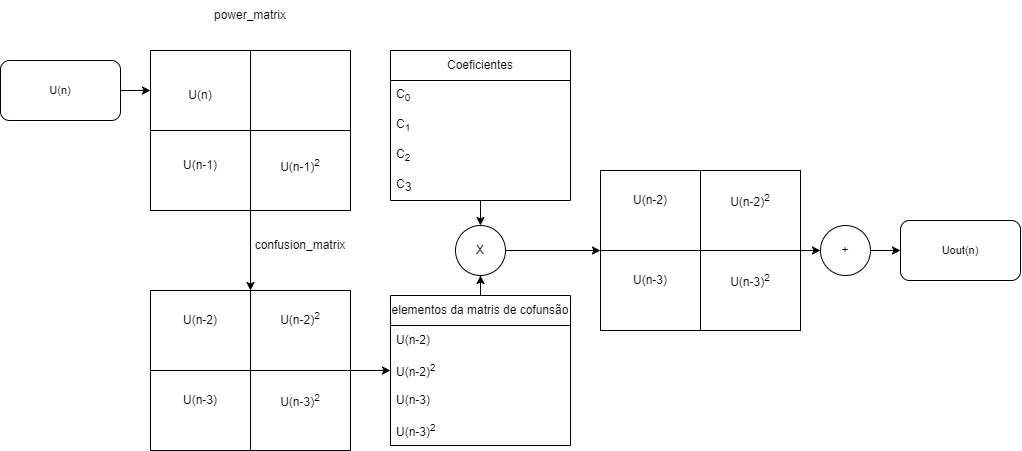
\includegraphics[width=\figsize]{fluxo_de_calculo.png}
	\caption{Processo de cálculo da saída}
	\label{fig:diagramaprocesssimpl}
\end{figure}

O resultado dessa implementação foi simulado em uma FPGA Virtex5 XC5VLX50T, utilizando um total de 150 registradores, 692 LUTs e 4 DSP48Es, operando a uma frequência de 61,44 MHz. A Figura \ref{fig:fpgasim} apresenta o resultado dessa implementação, representado pelos "x" em vermelho, em comparação com o resultado da simulação em Python, indicado pelos "." em azul.

\begin{figure}[htbp]
	\centering
	\captionsetup{justification=centering}
	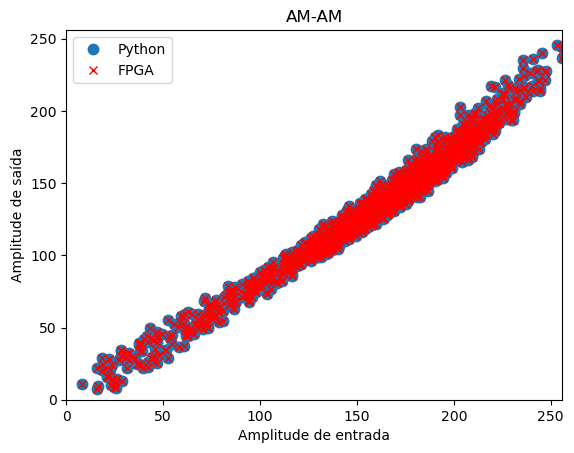
\includegraphics[width=\figsize]{fpgasim.png}
	\caption{Processo de cálculo da saída}
	\label{fig:fpgasim}
\end{figure}


\section{CONCLUSÃO}
A evolução dos sistemas de comunicação sem fio tem promovido a implementação de diversos serviços móveis, tornando essencial que esses sistemas operem com máxima eficiência. Nesse cenário, a implementação de um DPD em cascata com o PA surge como uma alternativa de baixo custo e interessante para melhorar o desempenho desses sistemas.
O objetivo deste trabalho de conclusão de curso é implementar em hardware um DPD baseado no modelo de Polinômio de Memória. Para isso, o projeto foi dividido em quatro etapas: estudo do DPD e da modelagem matemática, modelagem do DPD em software, implementação do DPD em hardware e, finalmente, design do circuito integrado.
Sendo assim a primeira etapa de desenvolvimento do projeto foi a modelagem do PA em virgula flutuante, utilizando o método do MP, para fazer essa modelagem utilizou-se um polinômio de 2° grau com uma amostra de memória, para fazer a validação dessa modelagem uitlizou-se a métrica do NMSE. Nesta etapa obteve-se um NMSE de -23,57 dB, a próxima etapa consiste em otimizar a quantidade de células lógicas utilizadas no processo limitando o número de bits utilizados. Nesta etapa observou-se que a partir de 8 bits, não havia melhora expressiva no NMSE, assim, essa foi a resolução em bits utilizadas para a amostragem de sinais. E por fim foi feito a modelagem do DPD em software o qual apresentou um comportamento inverso em relação o do PA, assim satisfazendo as necessidades.  Atualmente, o projeto está na etapa 3, que corresponde à implementação em hardware.  
Conclui-se, portanto, que o projeto alcançou os resultados esperados, com uma modelagem eficaz do PA e do DPD, satisfazendo os critérios de desempenho estabelecidos nas etapas iniciais.

\section*{REFERÊNCIAS}
\begingroup
\renewcommand{\section}[2]{}%

\begin{thebibliography}{}
	\bibitem{John2016} Elton John, ``Modelagem comportamental de amplificadores de potência de radiofrequência usando termos unidimensionais e bidimensionais de séries de Volterra", 2016.
	\bibitem{Kenington2000} Peter Kenington, ``High Linearity RF Amplifier Design", 2000.
	\bibitem{Cripps2006} Steve Cripps, ``RF Power Amplifiers for Wireless Communications", 2006.
	\bibitem{Chavez2018} Joel Huanca Chavez, ``Estudo comparativo entre as arquiteturas de identificação de pré-distorcedores digitais através das aprendizagens direta e indireta", 2018.
	\bibitem{Pedroni2010} Volnei Pedroni, ``Eletrônica Digital e VHDL ", 2010.
	\bibitem{Gonçalves2009} Eduardo Gonçalves de Lima and Giovanni Ghione, ``Behavioral modeling and digital base-band predistortion of RF power amplifiers", 2009.
	\bibitem{Schuartz2017} Luis Schuartz and Eduardo Lima, ``Polinômios com Memória de Complexidade Reduzida e sua Aplicação na Pré-distorção Digital de Amplificadores de Potência", 2017.
	
	\bibitem{Bonfim2016} Elton J Bonfim and Eduardo G De Lima, ``A Modified Two Dimensional Volterra-Based Series for the Low-Pass Equivalent Behavioral Modeling of RF Power Amplifiers", vol. 47, pp. 27-35, 2016.
\end{thebibliography}




\endgroup


\end{document}
